\section{Modelos de irradiancia solar}

Los modelos implementados para realizar la comparación de las mediciones son los siguientes:

\subsection{Irradiancia solar extraterrestre}

En el articulo de Djafer\cite{Djafer_2017} se menciona que utilizaron el modelo de irradiancia solar extraterrestre (GHI$_0$) para realizar comparaciones con sus mediciones. El modelo esta definido de la ecuacion \label{eq:GHI0}.

\begin{equation}
  \text{GHI}_0 = I_{SC}\left[ 1-0.033 cos\left( \frac{360n}{365}  \right)\right] cos(z)  \label{eq:GHI0}
\end{equation}

Donde $I_{SC}=1367$, la cual es la constante solar, n es el día consecutivo del año (n=1 es el primero y 365 el último) y $z$ es el ángulo zenital definido de la  siguiente manera:

\begin{equation}
  cos(z) = cos(\phi)cos(\delta)cos(\omega)+sin(\phi)sin(\delta)
\end{equation}

Donde $\phi,\delta,\omega$ son la latitud, declinación solar y el ángulo solar al momento de la medición.


\subsection{Declinación y ángulo solar}

La dependencia en el tiempo en la ecuacion \ref{eq:GHI0} vienen siendo introducidas por medio de la declinación solar y el ángulo solar, en la ecuación \ref{eq:declination} y \ref{eq:angle_solar} se encuentran definidas respectivamente.

\begin{equation}
  \delta = 24.45 sin(\gamma)
  \label{eq:declination}
\end{equation}

\begin{equation}
  \omega = 15(h_{LTC}-12)
  \label{eq:angle_solar}
\end{equation}

donde $h_{LTC}$ es la hora local y $\gamma$ es la fracción de rotación de la tierra con respecto al sol.

\subsubsection{Irradiancia solar global horizontal}

En el articulo de Kwarikunda\cite{Kwarikunda_2021} se menciona que realizaron comparaciones entre los modelos Berger-Duffle (B-D), Adnot-Bouges-Campana-Gicquel (A-B-C-G) y Robledo-Soler (R-S). Esto para obtener que modelo tiene una cercania menor a las mediciones a nivel del suelo en condiciones de cielo despejado. Llegando a que el modelo R-S fue el que obtiene un mejor rendimiento en la tarea. El modelo R-S se encuentra definido en la ecuación \ref{eq:rs_model}.

\begin{equation}
  GHI_{RS} = a(cos z)^b exp(-c(90-z))
  \label{eq:rs_model}
\end{equation}

donde $cos z$ es el angulo zenital antes definido y $a,b,c$ son constantes a determinar. En nuestro caso, estas constantes tienen los siguientes valores:

\begin{table}
  \centering
  \begin{tabular}{llll} \hline
    \textbf{Parametro }& \textbf{a} & \textbf{b} & \textbf{c} \\ \hline
    Valor     & 1119& 1.19 & 1x10$^{-6  }$\\ \hline
  \end{tabular}
  \label{table:rs_parameters}
  \caption{Parámetros del modelo R-S.}
\end{table}

\subsection{Comparación de los modelos}

Se realizo el calculo para el dia 8 de octubre de 2021 en la estación Noroeste. En la figura \ref{fig:comparison_models} se muestran los modelos GHI$_0$ y RS junto con la medición a nivel de suelo de la estación. En la cual se puede observar que existe una menor diferencia entre los modelos y la medición en la mañana y en la noche. El modelo RS obtiene una mejor aproximación a la medición en la estación.

\begin{figure}[H]
  \centering
  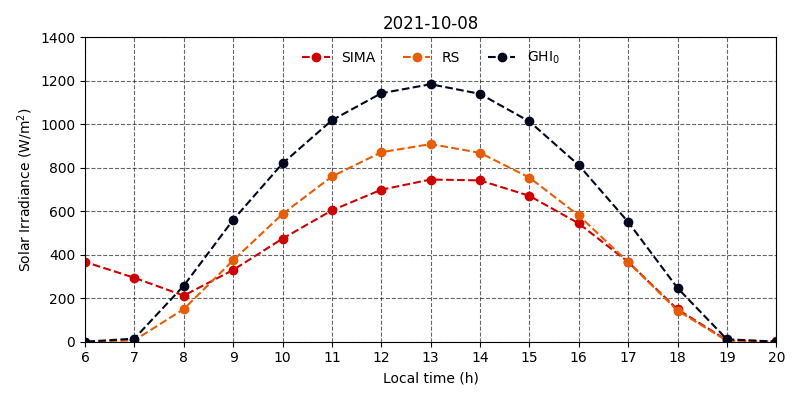
\includegraphics[width=14cm]{Graphics/2021-10-08.png}
  \caption{Comparación del modelo GHI$_0$, RS y la medición a nivel del suelo.}
  \label{fig:comparison_models}
\end{figure}

\section{Tratamiento de los datos}

A partir de las graficas diarias de la medición con los modelos, se centraron algunas mediciones con respecto al máximo solar, esto debido a que en algunas estaciones ocurria este error de forma esporpádica. Existian mediciones en los datos los cuales son imposibles físicamente, para ello se realizo una limpieza automatica de los datos. Esta limpieza consistia en eliminar aquellos valores que tuvieran una diferencia negativa con respecto al modelo GHI$_0$ o tuvieran una valor de k$_t$ (GHI/GHI$_0$) mayor a 0.8. Cuando el valor del modelo GHI$_0$ es 0 para una hora, este valor sera remplazado independientemente del criterio anterior. Esto debido a que representa un valor con ruido. Al termino de la limpieza, el tratamiento de los datos se enfoco en realizar una restauración de los mismos. Para ello se hizo uso de la similitud coseno (ecuación \ref{eq:cosine}).


\begin{equation}
  sim(m_i , m_j ) = \frac{m_i \cdot m_j}{||m_i|| ||m_j||}
  \label{eq:cosine}
\end{equation}

Se calculo la similitud coseno para mediciones de la misma estación, esto debido a que la topología alredor de cada una de ellas es diferente y esto puede ocasionar que existe una irregularidad si se toman todas a la vez. Para cada día se seleccionaron las primeras 30 mediciones que tuvieran una similitud más cercana a 1. Con estas mediciones seleccionadas se calculo el promedio horario, para así restaurar la mediciones con datos faltantes. En la figura \ref{fig:restoration} se muestran casos de restauración de datos en diferentes estaciones y días.

\begin{figure}[H]
  \centering
  \begin{subfigure}{15cm}
    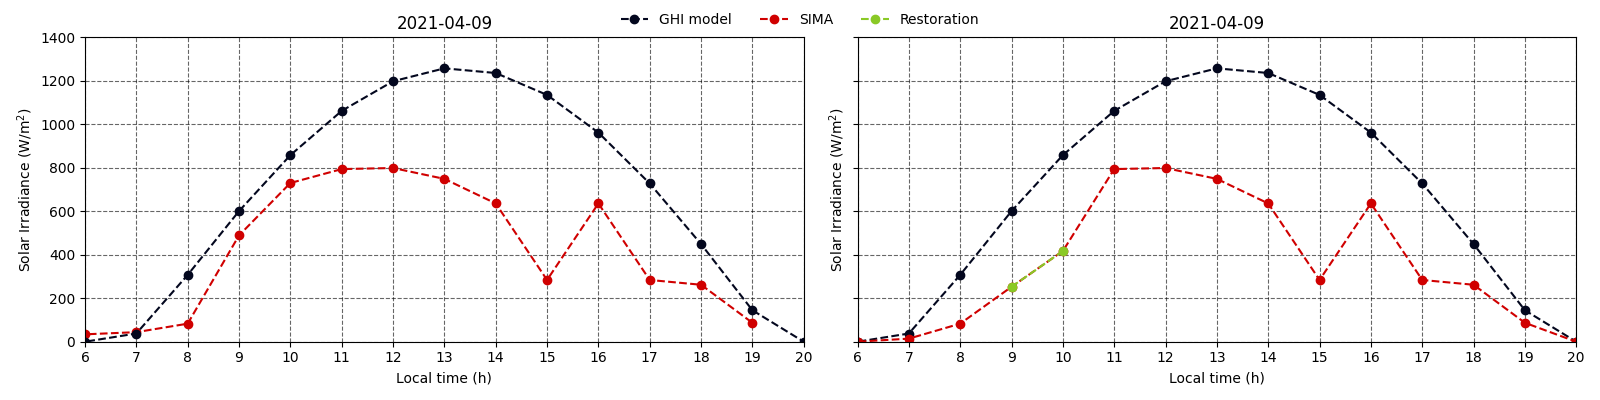
\includegraphics[width=15cm]{Graphics/2021-04-09.png}
  \end{subfigure}
  \begin{subfigure}{15cm}
    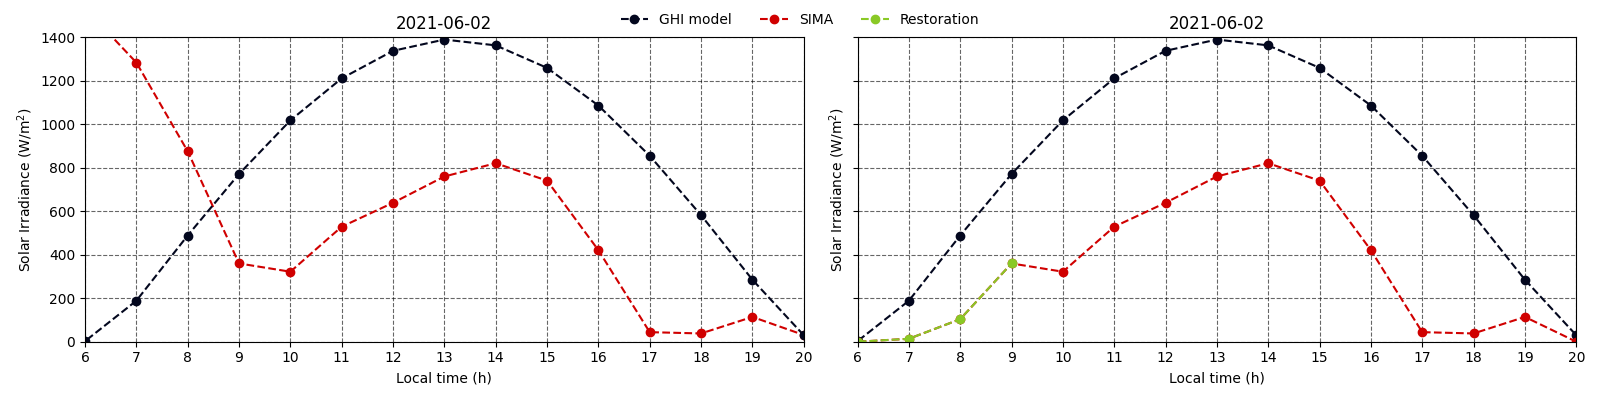
\includegraphics[width=15cm]{Graphics/2021-06-02.png}
  \end{subfigure}
  \begin{subfigure}{15cm}
    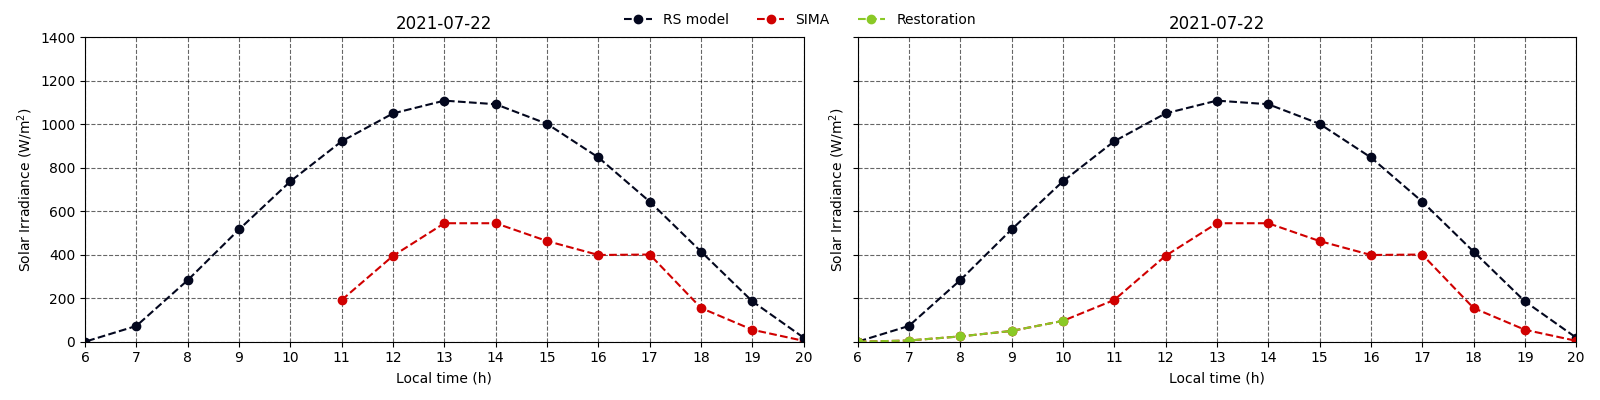
\includegraphics[width=15cm]{Graphics/2021-07-22.png}
  \end{subfigure}
  \begin{subfigure}{15cm}
    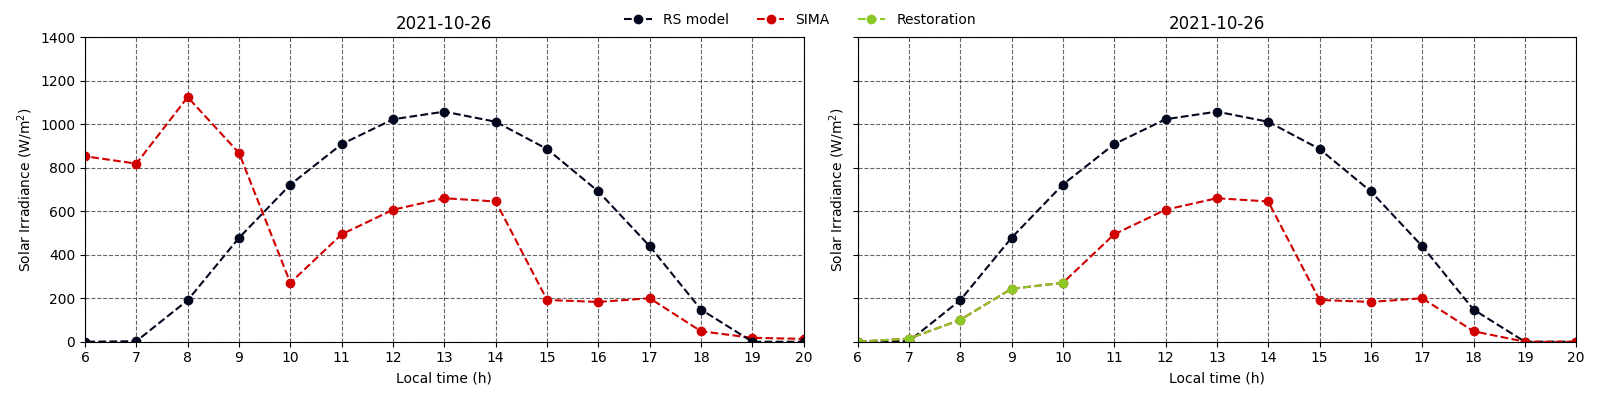
\includegraphics[width=15cm]{Graphics/2021-10-26.png}
  \end{subfigure}
  \caption{Restauracion de mediciones por medio de promerios horarios de las 30 mediciones más semejantes al día seleccioando}
  \label{fig:restoration}
\end{figure}

Con las mediciones restauradas se realizaron las comparaciones (diferencias y razones) con respecto a los modelos (GHI$_0$ y RS). Estas comparaciones seran usadas para entrenar a los modelos de clasificación clasicos y basados en redes neuronales.

\section{Modelos de clasificación clasicos}

Los modelos de clasificación clasicos que se implementaron son los siguientes:

\begin{itemize}
  \item Support Vector Machine (SVM)
  \item k-nearest neighbors (KNN)
  \item Random forest
  \item Gaussian naive
  \item Decision tree
\end{itemize}

Los cuales, el clasificador que mostro mejores resultados fue el random forest. Pero en general, usar los vectores de diferencias con respecto al modelo RS genera mejores resultados en comparación de los ratios y comparaciones basados en otros modelos.

\section{Modelos de redes neuronales}

Los modelos basados en redes neuronales a implementar son los siguientes

\begin{itemize}
  \item Perceptron
  \item RNN
  \item CNN (en duda)
  \item LSTM
\end{itemize}

Con este documento le adjunto los resultados obtenidos por los modelos clasificacion clasicos.
